\documentclass{warpdoc}
\newlength\lengthfigure                  % declare a figure width unit
\setlength\lengthfigure{0.158\textwidth} % make the figure width unit scale with the textwidth
\usepackage{psfrag}         % use it to substitute a string in a eps figure
\usepackage{rotating}
\usepackage{pstricks}
\usepackage[innercaption]{sidecap} % the cute space-saving side captions
\usepackage{scalefnt}
\usepackage{bm}
\usepackage{amsmath}
\usepackage{subcaption}

%%%%%%%%%%%%%=--NEW COMMANDS BEGINS--=%%%%%%%%%%%%%%%%%%%%%%%%%%%%%%%%%%
\newcommand{\alb}{\vspace{0.2cm}\\} % array line break
\newcommand{\efficiency}{\eta}
\newcommand{\ordi}{{\rm d}}
\newcommand{\unitvecdiff}[2]{\overline{\vec{#1} - \vec{#2}}}
%\let\vec\bf
\renewcommand{\vec}[1]{\bm{#1}}
\newcommand{\rhos}{\rho}
\newcommand{\Cv}{{C_{\rm v}}}
\newcommand{\Cp}{{C_{\rm p}}}
\newcommand{\Sct}{{{\rm Sc}_{\rm T}}}
\newcommand{\Prt}{{{\rm Pr}_{\rm T}}}
\newcommand{\nd}{{{n}_{\rm d}}}
\newcommand{\ns}{{{n}_{\rm s}}}
\newcommand{\nn}{{{n}_{\rm n}}}
\newcommand{\nr}{{{n}_{\rm r}}}
\newcommand{\ndm}{{\bar{n}_{\rm d}}}
\newcommand{\nsm}{{\bar{n}_{\rm s}}}
\newcommand{\turb}{_{\rm T}}
\newcommand{\mut}{{\mu\turb}}
\newcommand{\mfa}{\scriptscriptstyle}
\newcommand{\mfb}{\scriptstyle}
\newcommand{\mfc}{\textstyle}
\newcommand{\mfd}{\displaystyle}
\newcommand{\hlinex}{\vspace{-0.34cm}~~\\ \hline \vspace{-0.31cm}~~\\}
\newcommand{\hlinextop}{\vspace{-0.46cm}~~\\ \hline \hline \vspace{-0.32cm}~~\\}
\newcommand{\hlinexbot}{\vspace{-0.37cm}~~\\ \hline \hline \vspace{-0.50cm}~~\\}
\newcommand{\tablespacing}{\vspace{-0.4cm}}
\newcommand{\fontxfig}{\footnotesize\scalefont{0.918}}
\newcommand{\fontgnu}{\footnotesize\scalefont{0.896}}
\renewcommand{\fontsizetable}{\footnotesize\scalefont{0.9}}
\setcounter{tocdepth}{3}
\let\citen\cite

%%%%%%%%%%%%%=--NEW COMMANDS ENDS--=%%%%%%%%%%%%%%%%%%%%%%%%%%%%%%%%%%%%
%%%%%%%%%%%%%=--NEW COMMANDS BEGINS--=%%%%%%%%%%%%%%%%%%%%%%%%%%%%%%%%%%


\author{
  Bernard Parent 
}

\email{
  bernparent@gmail.com
}

\department{
  Aerospace and Mechanical Engineering
}

\institution{
  University of Arizona
}

\title{Lenard Air-Cesium Plasma Kinetics at High Temperature and Electric Field
}

\date{
  June 2020
}

%\setlength\nomenclaturelabelwidth{0.13\hsize}  % optional, default is 0.03\hsize
%\setlength\nomenclaturecolumnsep{0.09\hsize}  % optional, default is 0.06\hsize

\nomenclature{

  \begin{nomenclaturelist}{Roman symbols}
   \item[$a$] speed of sound
  \end{nomenclaturelist}
}


\abstract{
abstract
}

\begin{document}
  \pagestyle{headings}
  \pagenumbering{arabic}
  \setcounter{page}{1}
%%  \maketitle
  \makewarpdoctitle
%  \makeabstract
%  \tableofcontents
%  \makenomenclature
%  \listoftables
%%  \listoffigures










%
\begin{table}[t]
  \center\fontsizetable
  \begin{threeparttable}
    \tablecaption{Lenard high-temperature air-cesium chemical reactions.\tnote{a,b}}
    \label{tab:macheret}
    \fontsizetable
    \begin{tabular*}{\textwidth}{l@{\extracolsep{\fill}}lll}
    \toprule
    No.&Reaction & Rate Coefficient  & Refs. \\
    \midrule
    1  & $\rm O_2 + O_2  \rightarrow O+O+O_2$  
       &  $2.3\cdot 10^{19} \cdot {\cal A}^{-1}\cdot T^{-1}\cdot \exp(-59400/T)$~cm$^3$/s
       & \cite{misc:1964:lenard} \\
    2  & $\rm O_2 + O  \rightarrow O+O+O$  
       &  $8.5\cdot 10^{19}\cdot {\cal A}^{-1}\cdot T^{-1}\cdot \exp(-59400/T)$~cm$^3$/s
       & \cite{misc:1964:lenard} \\
    3  & $\rm O_2 + M_1  \rightarrow O+O+M_1$ 
       &  $3.0\cdot 10^{18}\cdot {\cal A}^{-1}\cdot T^{-1}\cdot \exp(-59400/T)$~cm$^3$/s
       & \cite{misc:1964:lenard} \\
    4  & $\rm N_2 + N_2  \rightarrow N+N+N_2$ 
       &  $3.8\cdot 10^{19}\cdot {\cal A}^{-1}\cdot T^{-1}\cdot \exp(-113200/T)$~cm$^3$/s
       & \cite{misc:1964:lenard} \\
    5  & $\rm N_2 + N  \rightarrow N+N+N$ 
       &  $1.3\cdot 10^{20}\cdot {\cal A}^{-1}\cdot T^{-1}\cdot \exp(-113200/T)$~cm$^3$/s
       & \cite{misc:1964:lenard} \\
    6  & $\rm N_2 + M_2  \rightarrow N+N+M_2$ 
       &  $1.9\cdot 10^{19}\cdot {\cal A}^{-1}\cdot T^{-1}\cdot \exp(-113200/T)$~cm$^3$/s
       & \cite{misc:1964:lenard} \\
    7  & $\rm NO + M_3  \rightarrow N+O+M_3$ 
       &  $2.4\cdot 10^{17}\cdot {\cal A}^{-1}\cdot T^{-0.5}\cdot \exp(-75500/T)$~cm$^3$/s
       & \cite{misc:1964:lenard} \\
    8  & $\rm O + N_2  \rightarrow N+NO$ 
       &  $6.8\cdot 10^{13}\cdot {\cal A}^{-1}\cdot  \exp(-37750/T)$~cm$^3$/s
       & \cite{misc:1964:lenard} \\
    9  & $\rm O + NO  \rightarrow N+O_2$ 
       &  $4.3\cdot 10^{7}\cdot {\cal A}^{-1}\cdot T^{1.5}\cdot \exp(-19100/T)$~cm$^3$/s
       & \cite{misc:1964:lenard} \\
    10  & $\rm N + O  \rightarrow NO^+ + e^-$ 
       &  $1.3\cdot 10^{8}\cdot {\cal A}^{-1}\cdot T \cdot\exp(-31900/T)$~cm$^3$/s
       & \cite{misc:1964:lenard} \\
    11  & $\rm O+O+O_2 \rightarrow O_2 + O_2 $  
       &  $1.9\cdot 10^{16}\cdot {\cal A}^{-2}\cdot T^{-1/2} $~cm$^6$/s
       & \cite{misc:1964:lenard} \\
    12  & $\rm O+O+O  \rightarrow O_2 + O$  
       &  $7.1\cdot 10^{16}\cdot {\cal A}^{-2}\cdot T^{-1/2} $~cm$^6$/s
       & \cite{misc:1964:lenard} \\
    13  & $\rm O+O+M_1  \rightarrow O_2 + M_1$ 
       &  $2.5\cdot 10^{15}\cdot {\cal A}^{-2}\cdot T^{-1/2} $~cm$^6$/s
       & \cite{misc:1964:lenard} \\
    14  & $\rm N+N+N_2  \rightarrow N_2 + N_2$ 
       &  $2\cdot 10^{18}\cdot {\cal A}^{-2}\cdot T^{-1} $~cm$^6$/s
       & \cite{misc:1964:lenard} \\
    15  & $\rm N+N+N  \rightarrow N_2 + N$ 
       &  $7\cdot 10^{18}\cdot {\cal A}^{-2}\cdot T^{-1} $~cm$^6$/s
       & \cite{misc:1964:lenard} \\
    16  & $\rm N+N+M_2  \rightarrow N_2 + M_2$ 
       &  $10^{18}\cdot {\cal A}^{-2}\cdot T^{-1} $~cm$^6$/s
       & \cite{misc:1964:lenard} \\
    17  & $\rm N+O+M_3  \rightarrow NO + M_3$ 
       &  $6\cdot 10^{16}\cdot {\cal A}^{-2}\cdot T^{-0.5} $~cm$^6$/s
       & \cite{misc:1964:lenard} \\
    18  & $\rm  N+NO \rightarrow O + N_2$ 
       &  $1.5\cdot 10^{13} \cdot {\cal A}^{-1} $~cm$^3$/s
       & \cite{misc:1964:lenard} \\
    19  & $\rm N+O_2 \rightarrow O + NO $ 
       &  $1.8\cdot 10^{8} \cdot {\cal A}^{-1} \cdot T^{1.5} \exp(-3020/T)$~cm$^3$/s
       & \cite{misc:1964:lenard} \\
    20  & $\rm  e^- + NO^+  \rightarrow N + O$ 
       &  $2\cdot 10^{19} \cdot {\cal A}^{-1} \cdot T_{\rm e}^{-1} $~cm$^3$/s
       & \cite{misc:1964:lenard} \\
    21 & $\rm e^- + O_2^+ \rightarrow O + O$  
       & $2.0 \cdot 10^{-7} \cdot (300/T_{\rm e})^{0.7}  $ cm$^3$/s
       & \cite{misc:1997:aleksandrov}\\
    22 & $\rm e^- + N_2^+ \rightarrow N + N$  
       & $2.8 \cdot 10^{-7} \cdot (300/T_{\rm e})^{0.5}  $ cm$^3$/s 
       & \cite{misc:1992:kossyi}\\
    23  & $\rm e^- + O   \rightarrow O^- + h_v$ 
       &  $7.2\cdot 10^{8}\cdot {\cal A}^{-1}$~cm$^3$/s
       & \cite{misc:1964:lenard} \\
    24  & $\rm e^- + O  + M_4  \rightarrow O^- + M_4$  
       &  $8.5\cdot 10^{19}\cdot {\cal A}^{-2}\cdot T_{\rm e}^{-0.5}$~cm$^6$/s
       & \cite{misc:1964:lenard} \\
    25 & $\rm e^- + O_2 +M_5 \rightarrow O_2^- + M_5$  
       &  ?
       &  BOLSIG+\\
    26 & $\rm e^- + O_2 +O_2 \rightarrow O_2^- + O_2$  
       &  $1.4 \cdot 10^{-29} \cdot \left( {300}/{T_{\rm e}}\right)\cdot  \exp \left( {-600}/{T}\right)$
       & \cite{misc:1992:kossyi}\\
    ~  &   
       & ~~~$\cdot \exp \left( {700 \cdot (T_{\rm e}-T)}/{(T_{\rm e} T)}  \right)$ cm$^6$/s
       & ~\\
    27 & $\rm e^- + O_2 + N_2 \rightarrow O_2^- + N_2$  
       & $1.07 \cdot 10^{-31} \cdot \left( {300}/{T_{\rm e}} \right)^2 \cdot \exp \left( {-70}/{T}\right)$          
       & \cite{misc:1992:kossyi}\\
    ~  &   
       & ~~~$\cdot \exp \left( {1500 \cdot (T_{\rm e}-T)}/({T_{\rm e} T})  \right)$ cm$^6$/s 
       & ~\\
    28  & $\rm  O^- + M_4 \rightarrow O + e^- + M_4$  
       &  $1.4\cdot 10^{12} \cdot {\cal A}^{-1} \cdot T \cdot \exp(-17016/T)$~cm$^3$/s
       & \cite{misc:1964:lenard} \\
    29 & $\rm O_2^{-} + M_6^{+} \rightarrow O_2 + M_6$ 
       & $2.0 \cdot 10^{-7} \cdot (300/T)^{0.5}$ cm$^3$/s
       & \cite{misc:1992:kossyi}\\
    30 & $\rm O_2^{-} + M_6^{+} + M_4\rightarrow O_2 + M_6 +M_4$ 
       & $2.0 \cdot 10^{-25} \cdot (300/T)^{2.5}$ cm$^6$/s  
       & \cite{misc:1992:kossyi}\\
    31  & $\rm O_2^- + O_2 \rightarrow e^- + O_2 + O_2$  
       & $8.6 \cdot 10^{-10} \cdot \exp \left( {-6030}/{T}\right)
               \left(1-\exp \left( {-1570}/{T} \right)  \right)$ cm$^3$/s
       & \cite{book:1997:bazelyan}, Ch.\ 2\\
    32  & $\rm e^- + N_2   \rightarrow N_2^+ + e^- + e^-$  
       &  ${\rm exp}(-0.0105809\cdot {\rm ln}^2 E^\star - 2.40411\cdot 10^{-75} \cdot {\rm ln}^{46}E^\star)$~cm$^3$/s
       & \cite{jcp:2014:parent} \\
    33  & $\rm e^- + O_2   \rightarrow O_2^+ + e^- + e^-$  
       &  ${\rm exp}(-0.0102785\cdot {\rm ln}^2 E^\star - 2.42260\cdot 10^{-75} \cdot {\rm ln}^{46}E^\star)$~cm$^3$/s
       & \cite{jcp:2014:parent} \\
    34  & $\rm e^- + NO   \rightarrow NO^+ + e^- + e^-$  
       &  ${\rm exp}(-5.9890\cdot 10^{-6} \cdot {\rm ln}^4 E^\star + 2.5988\cdot 10^{-84} \cdot {\rm ln}^{51}E^\star)$~cm$^3$/s
       & BOLSIG+ \\
    35  & $\rm  e^- + Cs  \rightarrow Cs^+ + e^- + e^-$  
       &  $1.6\cdot 10^{32} \cdot {\cal A}^{-1} \cdot T_{\rm e}^{-3.3} \cdot \exp(-45172/T_{\rm e})$~cm$^3$/s
       & \cite{misc:1964:lenard} \\
    36  & $\rm  e^- + Cs^+   \rightarrow Cs + h_v$  
       &  $7.2\cdot 10^{14} \cdot {\cal A}^{-1} \cdot T_{\rm e}^{-0.67}$~cm$^3$/s
       & \cite{misc:1964:lenard} \\
    37  & $\rm  e^- + Cs^+  + M_4 \rightarrow Cs + M_4$  
       &  $3.0\cdot 10^{19} \cdot {\cal A}^{-2} $~cm$^6$/s
       & \cite{misc:1964:lenard} \\
    38  & $\rm  e^- + Cs^+  + e^- \rightarrow Cs + e^-$  
       &  $4.0\cdot 10^{39} \cdot {\cal A}^{-2} \cdot T_{\rm e}^{-4.5} $~cm$^6$/s
       & \cite{misc:1964:lenard} \\
    39  & $\rm  Cs + O_2 \rightarrow Cs^+ + O_2^-$  
       &  $1.0\cdot 10^{17} \cdot {\cal A}^{-1} \cdot T^{0.07} \cdot \exp(-39836/T)$~cm$^3$/s
       & \cite{misc:1964:lenard} \\
    40  & $\rm  Cs + O \rightarrow Cs^+ + O^-$  
       &  $8.7\cdot 10^{16} \cdot {\cal A}^{-1} \cdot T^{-0.15} \cdot \exp(-28177/T)$~cm$^3$/s
       & \cite{misc:1964:lenard} \\
    41  & $\rm  Cs + M_4 \rightarrow Cs^+ + e^- + M_4$  
       &  $1.2\cdot 10^{12} \cdot {\cal A}^{-1} \cdot T^{1.18} \cdot \exp(-45172/T)$~cm$^3$/s
       & \cite{misc:1964:lenard} \\
    42  & $\rm  Cs + NO^+ \rightarrow Cs^+ + NO$  
       &  $6.02\cdot 10^{13} \cdot {\cal A}^{-1} \cdot T^{-0.5}$~cm$^3$/s
       & \cite{misc:1964:lenard} \\
    43  & $\rm  Cs^+ + O_2^-\rightarrow Cs + O_2 $  
       &  $2.0\cdot 10^{17} \cdot {\cal A}^{-1} $~cm$^3$/s
       & \cite{misc:1964:lenard} \\
    44  & $\rm  Cs^+ + O^- \rightarrow Cs + O$  
       &  $2.0\cdot 10^{19} \cdot {\cal A}^{-1} \cdot T^{-0.6} $~cm$^3$/s
       & \cite{misc:1964:lenard} \\
    45  & $\rm  Cs^+ + NO \rightarrow Cs + NO^+$  
       &  $8.07\cdot 10^{11} \cdot {\cal A}^{-1} \cdot \exp(-61800/T)$~cm$^3$/s
       & \cite{misc:1964:lenard} \\
    \bottomrule
    \end{tabular*}
\begin{tablenotes}
\item[{a}] Notation and units: ${\cal A}$ is Avogadro's number set to $6.02214 \times 10^{23}$ mol$^{-1}$; $E^\star$ is the reduced effective electric field ($E^\star\equiv|\vec{E}|/N$) in units of V$\cdot$m$^2$; $T_{\rm e}$ is the electron temperature in Kelvin; $T$ is the neutrals temperature in Kelvin.
\item[{1}] $\rm M_1=N,~N_2,~NO,~NO^+$
\item[{2}] $\rm M_2=O,~O_2,~NO,~NO^+$
\item[{3}] $\rm M_3=O,~O_2,~N,~N_2,~NO^+$
\item[{4}] $\rm M_4=O,~O_2,~N,~N_2,~NO$
\item[{5}] $\rm M_5=O,~N,~NO$
\item[{6}] $\rm M_6=O_2,~N_2,~NO$

\end{tablenotes}
   \end{threeparttable}
\end{table}
%



\begin{figure}[!t]
  \centering
        \begin{subfigure}{0.49\textwidth}
            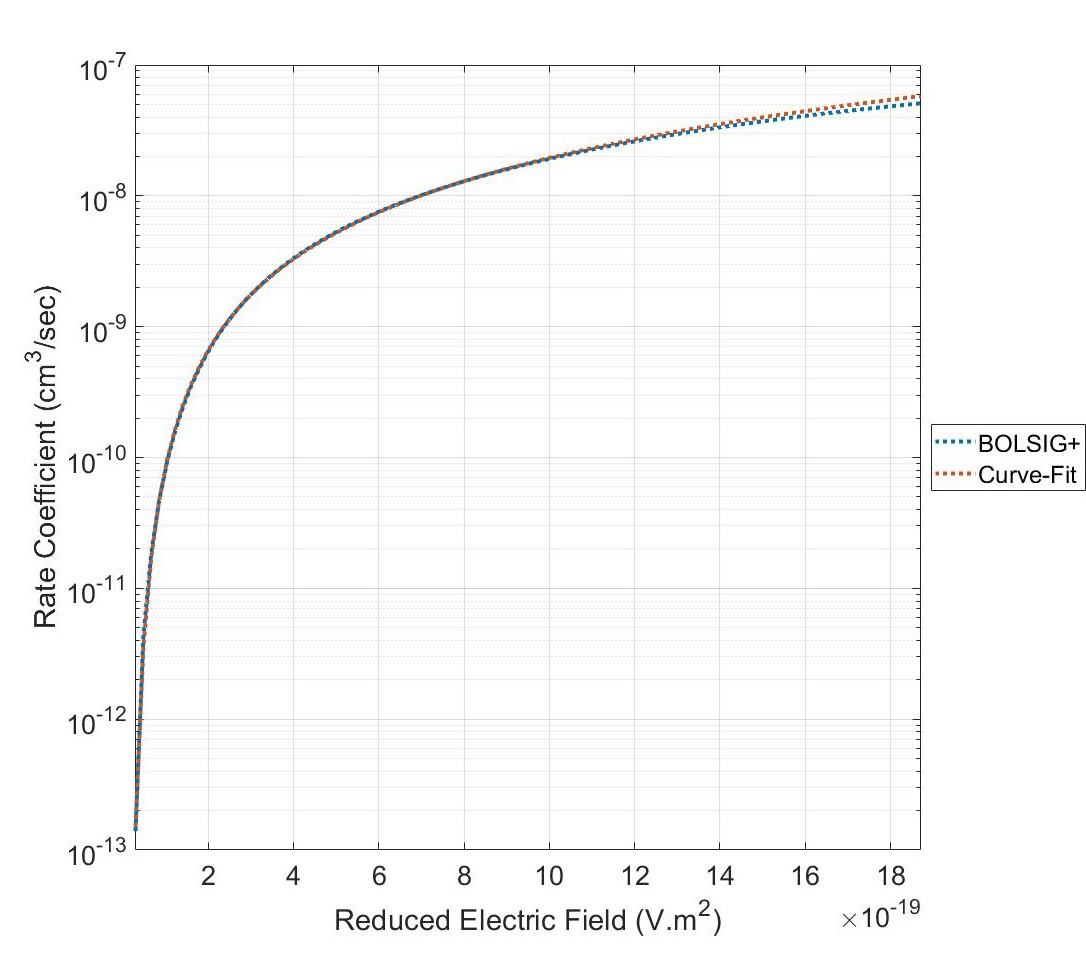
\includegraphics[width=0.99\linewidth]{NO_1.jpg}
            \caption{ Reaction 22: $\rm e^- + NO   \rightarrow e^- + e^- + NO^+ $. In the $E/N$ range 3 $\cdot$ 10$^{-20}$ to 187$\cdot$ 10$^{-20}$ V$\cdot$m$^2$, the maximum relative error between the BOLSIG+ data and the curve fit is of 14.9\% and the mean error is of 4.04\%.}
        \end{subfigure}
% \caption{Average heat flux to the wall and skin friction during the $1^{st}$, $3^{rd}$, $5^{th}$ and $20^{th}$ period.}

\end{figure}







\bibliographystyle{warpdoc}
\bibliography{all}


\end{document}



